\section{Theorie}
Das Ziel dieses Versuches ist es, die Kristallstruktur und die Größe der Einheitszelle
von zwei verschiedenen Probematerialien zu bestimmen, indem Debye-Scherrer-Aufnahmen
angefertigt werden.

\subsection{Beschreibung von Kristallstrukturen}
Ein Großteil der kondesierten Materie liegt in kristalliner Struktur vor.
Um diese Struktur aufzulösen, muss die räumliche Auflösung der Messvorrichtung in der
gleichen Größenordnung liegen wie die Abstände zwischen den Atomen. Dafür eignen sich
neben langsamen Neutronen oder Elektronen auch Röntgenstrahlen. Die im Folgenden
beschriebene Methode basiert auf der Beugung von Röntgenstrahlung an der Kristallstruktur.

Die räumliche Beschreibung der Kristalle lässt sich aus zwei Elementen zusammensetzen:
der Basis und des Punktgitters. Zusammen ergeben sie die Kristallstruktur, wie in
\autoref{abb:struktur} dargestellt.
\begin{figure}
  \centering
  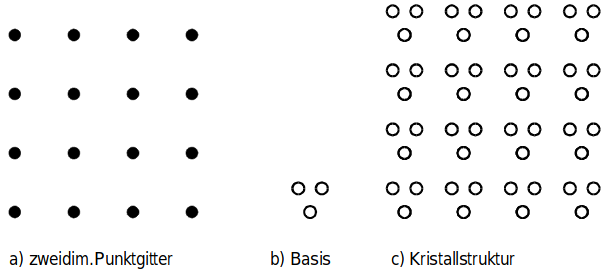
\includegraphics[scale=0.5]{content/pics/basis_gitter.png}
  \caption{Bestandteile der Kristallstruktur. \cite{anleitung}}
  \label{abb:struktur}
\end{figure}
Die Basis besteht dabei entweder aus einem Atom oder einer Atomgruppe. Um die verschiedenen
Punktgitter zu klassifizieren, werden durch drei Vektoren $\vec{a}, \vec{b}$ und $\vec{c}$
fundamentale Translationen aufgespannt, die durch
\begin{equation}
  \vec{t} = n_1 \, \vec{a} + n_2 \, \vec{b} + n_3 \ \vec{c} \qquad \text{mit} \ n_i \in \mathbb{N}
  \label{eqn:1}
\end{equation}
definiert sind. Mithilfe dieser Vorschrift lässt sich das ganze Gitter aufspannen, da
alle Punkte, die sich mit \eqref{eqn:1} darstellen lassen, Gitterpunkte sind.

Ein weitere Größe, die bei der Beschreibung von Kristallstrukturen von Bedeutung
ist, ist die Elementarzelle.  Diese ist definiert als die kleinste Einheit, durch
welche die Kristallstruktur vollständig festgelegt ist. Falls in dem von den Vektoren
aus \eqref{eqn:1} aufgespannte Parallelepiped nur in den acht Eckpunkten Atome sitzen,
dann ist diese Elementarzelle primitiv. Sie enthält nur ein Atom. Allerdings lässt sich
die Kristallstruktur nicht mehr vollständig aus vielen primitiven Elementarzellen
aufbauen, falls die Basis aus mehr als einem Atom besteht, da in diesem Fall die Atome
nicht nur in den Eckpunkten des Parallelepipeds sitzen.

Im nachfolgenden Versuch werden verschiedene kubische Strukturen untersucht.
Eine davon ist die kubisch-raumzentrierte Struktur (\textit{eng.} bcc (body centered cubic)).
Diese besitzt zwei Atome pro Elementarzelle. Eine Darstellung ist in \autoref{abb:elementarzelle_kubisch}
zu finden.
\begin{figure}
  \centering
  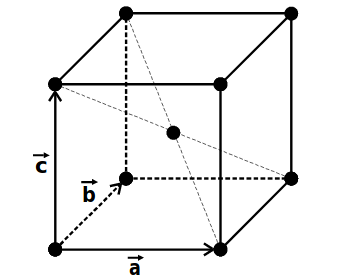
\includegraphics[scale=0.5]{content/pics/elementarzelle_kubisch.png}
  \caption{Schematische Darstellung der Elementarzelle des kubisch-raumzentrierten
  Gitters. \cite{anleitung}}
  \label{abb:elementarzelle_kubisch}
\end{figure}
Im Koordinatensystem der Elementarzelle liegen die Atome bei
\begin{equation}
  (0, 0, 0) \ \text{und} \ (\frac{1}{2}, \frac{1}{2}, \frac{1}{2}) \, .
  \label{eqn:atome-raumzentriert}
\end{equation}
Die acht nächsten Nachbarn haben einen Abstand untereinander von
$\frac{1}{2} \sqrt{3} a$, mit $a$ als Kantenlänge des Würfels.

Im Gegensatz zur kubisch-raumzentrierten Struktur gibt es bei der kubisch-flächenzentrierten
(\textit{eng.} fcc (face centered cubic)) Struktur statt des zentralen Atoms in der
Mitte des Würfels jeweils ein Atom in der Mitte der Seitenflächen des Würfels, wie
in \autoref{abb:elementarzelle_flaeche} zu sehen.
\begin{figure}
  \centering
  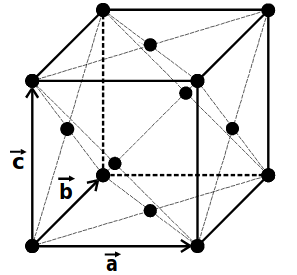
\includegraphics[scale=0.5]{content/pics/elementarzelle_flaeche.png}
  \caption{Schematische Darstellung der Elementarzelle des kubisch-flächenzentrierten
  Gitters. \cite{anleitung}}
  \label{abb:elementarzelle_flaeche}
\end{figure}
Die Atome der Elementarzelle liegen bei
\begin{equation}
  (0, 0, 0), (\frac{1}{2}, \frac{1}{2}, 0), (\frac{1}{2}, 0, \frac{1}{2}) \ \text{und}
  \ (0, \frac{1}{2}, \frac{1}{2}) \, .
  \label{eqn:atome-flaechenzentriert}
\end{equation}
Die zwölf nächsten Nachbarn haben einen Abstand von $\frac{1}{2} \sqrt{2} a$
untereinander.
% cleares the page and appends all not yet used floats at the beginning of the
% next page
\pagebreak
\subsection{Millersche Indizes und Abstandsberechung}

Eine wichtige Größe für diesen Versuch sind die Millerschen Indizes. Diese kennzeichnen
die Lage der Netzebenen im Kristall relativ zum Koordinatensystem des Kristalls,
welche definiert sind als Ebene, in der die Schwerpunkte der Atome liegen.
Die Millerschen Indizes, meist mit h, k und l bezeichnet, sind die Zahlenwerte,
die sich errechnen, wenn die Schnittpunkte der Netzebene mit den Koordinatenachsen
gebildet und die reziproken Werte genommen werden. Um gebrochenen Zahlen zu vermeiden,
wird das Zahlentripel mit den Inversen der gebrochenen Zahlen multipliziert. Nach
Definition werden negative Achsenabschnitte durch einen Strich über dem jeweiligen Index
gekennzeichnet. Falls eine Netzebene parallel zu einer Achse liegt, dann ist der Millersche
Index 0, da der Schnittpunkt mit der Koordinatenachse im Unendlichen liegt.

Die Millerschen Indizes sind unter anderem deswegen eine zentrale Größe in der Beschreibung
von Kristallstrukturen, da aus ihnen relativ einfach der Abstand benachbarter Netzebenen
berechnen lässt. In \autoref{abb:abstand} ist eine Skizze zur Berechnung zu sehen.
\begin{figure}
  \centering
  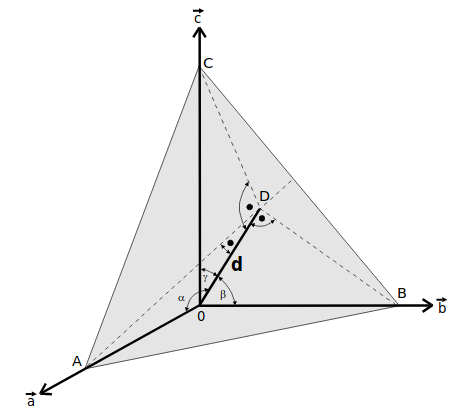
\includegraphics[scale=0.5]{content/pics/netzebenenabstand.png}
  \caption{Grafische Darstellung der wichtigsten Größen zur Berechnung des Netzebenenabstandes
  aus den Millerschen Indizes. \cite{anleitung}}
  \label{abb:abstand}
\end{figure}
Da der Netzebenabstand $d$ senkrecht auf den beiden Netzebenen(eine mit den Punkten
A, B und C und eine mit dem Ursprung), sind die Dreiecke ODA, ODB und ODC rechtwinklig.
Aus trigonometrischen Beziehungen ergibt sich
\begin{equation}
  d = \left(\sqrt{\frac{h^2}{a^2} + \frac{k^2}{b^2} + \frac{l^2}{c^2}}\right)^{-1}
  \label{eqn:abstand}
\end{equation}
und für kubische Systeme mit $a = b = c$ wird \eqref{eqn:abstand} zu
\begin{equation}
  d = \frac{a}{\sqrt{h^2 + k^2 + l^2}} \, .
  \label{eqn:abstand_kubisch}
\end{equation}
\pagebreak
\subsection{Beugung von Röntgenstrahlen an Kristallen}

Die Wechselwirkung der Röntgenstrahlung mit den
Elektronen und Atomkernen des Kristalls findet als klassischer Streuprozess
von elektronmagnetischen Wellen statt. Dadurch, dass die Atome in einem Kristall
periodisch angeordnet sind, sind die gestreuten Wellen interferenzfähig und je nach
Raumrichtung löschen sich diese aus oder verstärken sich. Damit kann eine Strukturbestimmung
des Kristalls durchgeführt werden. \\
Die Atomkerne und Elektronen, an denen gestreut wird, verhalten sich unter Einwirkung der
Röntgenstrahlung als Hertzscher Dipol mit der emittierten Intensität
\begin{equation}
  I_e(r, \theta) = I_0 \left(\frac{\symup{\mu_0} \, q^2}{4 \, \pi \, m} \right)^2 \frac{1}{r^2}
  \frac{1 + \cos^2(2\theta)}{2} \, .
  \label{eqn:hertz}
\end{equation}
Dabei ist $I_0$ die ursprüngliche Intensität der Welle, $\symup{\mu_0}$ die magnetische
Feldkonstante, $r$ der Abstand zwischen Aufpunkt und Teilchen und $2\theta$ der Winkel
zwischen einfallendem und gestreutem Strahl. Aus \eqref{eqn:hertz} wird ersichtlich, dass
die Masse der Atomkerne so groß ist, dass die Streuung vernachlässigt werden kann.
Da die Elektronen im Kristall nicht isoliert, sondern in Hüllen um die Atomkerne anliegen
und die Ausdehnung der Elektronenhüllen in der Größenordnung der Wellenlänge der
verwendeten Röntgenstrahlung liegt, schwingen nicht alle getroffenen Elektronen
in Phase. Das führt dazu, dass die vom Atom gestreute Intensität geringer ist
als die Intensität, die gegeben wäre, falls die Ausdehnung der Elektronenhülle
klein gegen die Wellenlänge der Röntgenstrahlung ist. In diesem Fall wird in \eqref{eqn:hertz}
der quadrierte Bruch durch
\begin{equation}
    \left(\frac{\symup{\mu_0} (z \symup{e_0})^2}{4 \, \pi \, z \, \symup{m_e}} \right)^2 \, ,
    \label{eqn:hertz-angepasst}
\end{equation}
mit $z$ als Ordnungszahl, $\symup{e_0}$ und $\symup{m_e}$ als Ladung bzw.
Masse eines Elektrons. Damit wird eine wichtige Größe in der Festkörperpyhsik
definiert, der Atomformfaktor
\begin{equation}
  f^2 = \frac{I_a}{I_e}
  \label{eqn:atomformfaktor}
\end{equation}
mit $I_a$ als Atomstreuintensität und $I_e$ als Streuintensität eines Einzelelektrons.
$f$ ist somit abhängig von der Ordnungszahl, der Wellenlänge der Röntgenstrahlung
und der Streurichtung. Zur genaueren Berechnung von $f$ muss die Elektronendichteverteilung
$\rho(\vec{r})$ benutzt werden, da punktförmige Elektronen eine zu grobe Näherung sind.
Nach einem Integral über die Elektronenhülle und Symmetrieüberlegungen mit dem Wellenzahlvektor
ergibt sich, dass $f$ für verschiedene Atome und Ionen meist als Funktion von $z$
und $\sin(\theta)/\lambda$ angegeben wird. \\
Um die Betrachtung der Streuung von Röntgenstrahlung an Elektronen weiter auf die Streuung
an Kristallen anzupassen, muss auch die Streuung an der Elementarzelle eines Kristalls
betrachtet werden. Auch in diesem Fall treten aufgrund der festen räumlichen Verteilung
in einem Kristall Interferenzeffekte auf. Wenn der Phasenunterschied zwischen den
gestreuten Wellen der verschiedenen Atomen in der Elementarzelle betrachtet und phasenrichtig
summiert wird, ergibt sich
\begin{equation}
  S = \sum_j f_j \, \symup{e}^{-2 \pi \symup i \,(x_j \, \vec{a} + y_j \, \vec{b}
  + z_j \, \vec{c})(\vec{k} - \vec{k}_0)} \, I_e
  \label{eqn:strukturfaktor-allgemein}
\end{equation}
als Strukturamplitude der Elementarzelle mit $f_j$ als Atomfromfaktoren der
einzelnen Atome, $\vec{r}_j = x_j \, \vec{a} + y_j \, \vec{b}
+ z_j \, \vec{c}$ als Ortsvektor der Atome in der Elementarzelle ausgedrückt durch
die Basisvektoren der Elementarzelle ($|x_j|, |y_j|, |z_j| \leq 1$) und $\vec{k}$
bzw. $\vec{k}_0$ als Wellenzahlvektoren der gestreuten bzw. der einfallenden Welle.
Der Strukturfaktor $SS*$ gibt das Verhältnis zwischen der Intensität der Streuung an
der Elementarzelle und der Streuung an einem einzelnen Elektron an. \eqref{eqn:strukturfaktor-allgemein}
muss noch angepasst werden, da $\vec{k}$ bzw. $\vec{k}_0$ in einem Kristall nicht frei
wählbar sind, wenn eine nicht verschwindene Intensität gestreut werden soll, da
die Elementarzellen in einem festen Kristallgitter angeordnet sind. Die Auslöschung
tritt aufgrund von Interferenzeffekten auf, da an mehreren tausend untereinander liegenden
Netzebenen gestreut wird. Ein gestreuter Röntgenstrahl ist somit nur zu beobachten, falls
die Braggsche Bedingung
\begin{equation}
  n \, \lambda = 2 \, d \, \sin(\theta)
  \label{eqn:bragg}
\end{equation}
mit $n \in \mathbb{N}$ erfüllt ist. Sie folgt aus geometrischen Überlegungen
und Additionstheoremen. \\
Die Bragg Bedingung lässt sich auch durch reziproke Gittervektoren ausdrücken. Dabei
sind reziproke Gittervektoren die \enquote{normalen} Gittervektoren im Impulsraum.
Diese reziproken Gittervektoren lassen sich mit den Millerschen Indizes ebefalls
einer Netzebene zuordnen und damit ergibt sich für die Strukturamplitude \eqref{eqn:strukturfaktor-allgemein}
\begin{equation}
  S(h, k, l) = \sum_j f_j \, \symup e^{-2\pi \symup i (x_j \, h + y_j \, k + z_j \, l)} \, .
  \label{eqn:strukturfaktor-final}
\end{equation}
Mit \eqref{eqn:strukturfaktor-final} kann nun errechnet werden, für welche Elementarzellen
an welchen Ebenen Röntgenreflexe auftreten oder nicht. Dies ist ein zentraler Bestandteil
der Auswertung.

\section{Durchführung}
Im Folgenden werden der experimentelle Aufbau und die Versuchsdurchführung beschrieben.
\subsection{Aufbau}
In \autoref{abb:aufbau} ist der Versuchsaubau schematisch dargestellt.
\begin{figure}
  \centering
  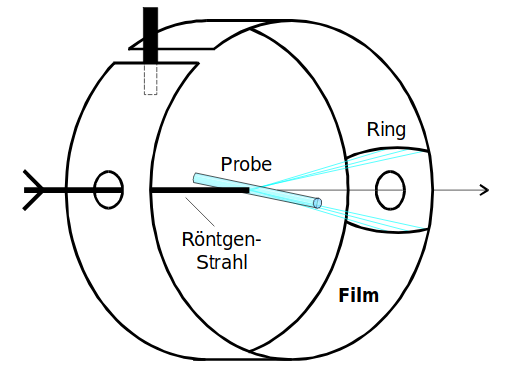
\includegraphics[scale=0.5]{content/pics/aufbau.png}
  \caption{Schematische Darstellung des Versuchsaufbaus. \cite{anleitung}}
  \label{abb:aufbau}
\end{figure}
Die Probe befindet sich in einem Ring aus Fotofilm und wird von monochromatischer
Röntgenstrahlung bestrahlt. Die Probe ist dabei fein pulversisiert und wird in zylindrische
Form gebracht, damit in jeder Raumrichtung einige Kristallite in Reflexionsrichtung
zur Einstrahlrichtung stehen. Die von der Probe unter dem Winkel $\theta$ gebeugte
Strahlung liegt auf einem
Kegelmantel mit dem Öffnungswinkel $2\theta$ aufgrund der statistischen Verteilung der
Orientierung der Kristalle in der Probe. Die entstehenden Kegelschnitte auf dem Filmstreifen
lassen sich durch Kreise annähern, deren Radius proportional zum Beugungswinkel ist.
In der Grafik nicht zu sehen ist der Motor, der die Probe während der Messung um ihre
Längsachse dreht, damit die \enquote{Debye-Ringe} gleichmäßig geschwärzt werden.
\subsection{Versuchsdurchführung}
Als erstes wurde eine Leermessung durchgeführt, um den Aufbau und die Funktionsweise
kennenzulernen und zu testen. Dann wurde eine Metallprobe hergestellt, indem
mit Vaseline eine feinkörnigen Metallprobe um ein Glasröhrchen herum verteilt wird.
Daraufhin wird das Behältnis mit dem Filmstreifen präpariert und ein eventuelles
unregelmäßiges Drehen der Probe ausgeglichen. Dann wird die leere Probe eine Stunde,
die Metallprobe zwei Stunden und die Salzprobe vier Stunden mit Röntgenstrahlung
bestrahlt. Abschließend werden die Filme entwickelt.
